\documentclass[a4paper,english,11pt,]{scrartcl}
\usepackage{mystyle}
\usepackage{rotfloat}
\title{Traveling Salesman Problem}
\subtitle{Genetic Algorithms and Evolutionary Computing (|H08M3a|)}
\author{Li Quan\and Wout Swinnen}
%\subject{Verslag}
\date{January 13, 2011}
\bibliographystyle{abbrv}

\begin{document}
\maketitle

%\begin{abstract}

%\end{abstract}
\small{
\tableofcontents
\listoffigures
\listoftables
}


\clearpage

\section{Introduction}
In this project, some of the key concepts of solving combinatorial optimization problems with the use of genetic algorithms are explored. To be more precise, we will implement genetic operators and investigate their characteristics when applied to the traveling salesman problem (TSP). 


\section{Traveling salesman problem}
\subsection{Description}
The TSP is the classic example of a route planning problem. The aim of the TSP is to find a route between cities that is as short as possible, where every city has to be visited once, and where the final city has to be the same one as the starting city. There are many more complicated forms of this TSP, e.g.,~\cite{affenzeller2009genetic,multiple_tsp,gutin2002traveling}, but these will not be discussed in this project.
% 
% \subsection{Genetic algorithm}
% The genetic algorithm (GA) is an elegant solution to this problem, among many other problems. It is a concept that has grown over the last half century, which mimics the mechanisms of natural evolution and genetics as known from biology. Just like our genes, genetic algorithms tend to make sure the strongest solutions to a problem survive, and the weaker ones do not. To do so, it makes use of genetic operators such as crossover and mutation, and often also a selection process comes at hand. 

\subsection{TSP representation}
First, we will discuss how to represent a TSP tour. This will have an impact on the possible crossover and/or mutation operators and their performance.

\subsubsection{Adjacency representation}
% It is easily seen that by varying different solution parameters, the outcome of the genetic process will differ greatly. For example, when observing a natural evolution situation, the effects of population size on the genetic diversity among the animals is obvious. The same accounts for genetic algorithms, where the tweaking of the solution parameters is of utmost importance for acquiring strong results. 
% By running the program repeatedly experimenting with different parameter values, many conclusions can be drawn by studying the population and its dynamics. Parameters that have great influence on the performance are for example the population size, the number of generations allowed, the mutation probability, the crossover probability and the percentage of elitism solutions kept (juist?). 
% As for the size of the solutions population and the number of generations, it speaks for itself that increase of these parameters will improve the solution quality, but the computational effort will also increase with them. That’s why a compromise between these two should be found. A bigger population in each generation will allow more diversity within the population, and thus a wider spread among the search space, whereas a larger number of consecutive generations will allow a deeper search for locally optimal solutions. 
% Crossover probability will also affect the wideness of the search for solutions. As crossover introduces disorder and makes great changes to the genotype of the individuals, a greater probability will boost the genetic diversity among the population. This will allow a more diffuse exploration of the search space, and the general optimum will more likely be found. However, when the probability of crossover gets too high, it will also inhibit a more profound search for local optima. This is opposed to mutation, which makes mere small changes to the genotype, and a greater probability of mutation will aid in local fitness optimization. 
% Wat is die elite precies? Is het parent selection? Offspring selection?  Het is toch parent selection he? Anders heb ik beneden nog wat foutjes gezegd bij de selection operators.
% It speaks for itself that the use of heuristics such as a loop detection method will generally improve performance.

The adjacency representation describes a tour with a list of $n$ cities where city $j$ is listed in position $i$ if and only if the tour leads from city $i$ to city $j$. The adjacency representation allows schemata analysis, but it has many disadvantages. The use of normal crossover operators will very likely introduce illegal tours in the population, and they have to be complemented with repair operators. On the other hand, the use of crossover operators designed for the adjacency representation will generally lead to very poor results. 

 %Because of its global poor performance, we will not discuss this representation to its full extent, and replace it with another, namely the path representation. 

\subsubsection{Ordinal representation}
When using the ordinal presentation, a tour is also represented as a list of $n$ cities; the $i$th element of the list is a number
in the range from 1 to $n - i + 1$, and there an ordered list of cities serving as a reference point is also used. 

The main advantage of this rather complicated ordinal representation lies in the fact that the classical crossover can be used. (This follows from the fact that the $i$th element of the tour representation is always a number in the range from 1 to $n -i + 1$.) The results obtained using ordinal representation however have been generally poor. 


\subsubsection{Path representation}
The most straightforward, natural representation for describing TSP tours is the path representation. In the path representation, once again a list of $n$ cities is used. In this list, the $j$th element with value $i$ denotes that the $j$th city to be visited is city $i$. Also in this case, the classical crossover operators will not be usable. 
However using this representation, specific crossover operators have been designed that do give very good results.

\subsection{Tasks}

The main objective of this project is to investigate the performance of various GA operators and discuss possible improvements. 
In particular, we change the original adjacency representation (with alternating edge crossover and simple inversion\footnote{In the original implementation this was somewhat confusingly named inversion mutation, which is a slightly more complicated variant.} mutation) to \emph{path representation} and implement appropriate operators. We implemented all crossover and mutation operators mentioned in \cite{affenzeller2009genetic} for the path representation. 

More specifically, this consists of the following crossover operators: \emph{Partially Matched Crossover (PMX)}, \emph{Order Crossover (OX)}, \emph{Cyclic Crossover (CX)} and \emph{(Enhanced) Edge Recombination Crossover ((E)ERX)}; and the following mutation operators:  \emph{inversion}, \emph{exchange} and \emph{insertion} mutation. 

As an optional task, we have chosen to analyze the selection processes of \emph{proportional (roulette wheel)} and \emph{tournament} selection. 

These operators and processes will be tested by comparing solution speeds, minimal tour distances, genetic diversity, etc.
Finally, we will also briefly compare with some alternative approaches to solve TSP problems.

\subsection{Benchmark problems}
In general, the optimal solution of TSP problems is not known a priori. However, to study the performance of the algorithms it is crucial to have several benchmark problems with a known optimal solution in order to establish a baseline.


\begin{figure}[hbtp]
\centering
\subfloat[\dataset{belgiumtour} (?)]{\label{fig:belgiumtour}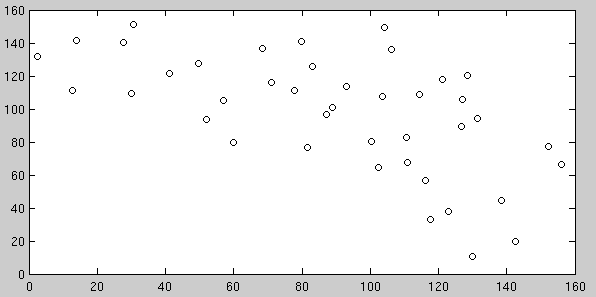
\includegraphics[width=0.32\textwidth]{belgiumtour}} \vspace{0.5cm}
\subfloat[\dataset{bcl380} (564)]{\label{fig:bcl380}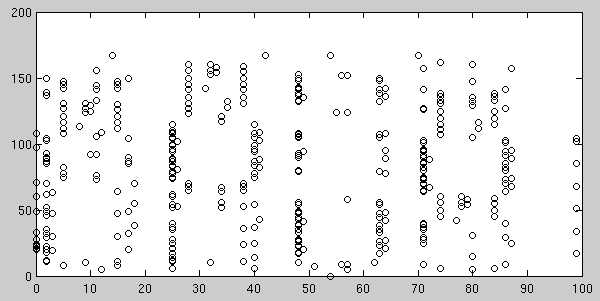
\includegraphics[width=0.32\textwidth]{bcl380}}                \vspace{0.5cm}
\subfloat[\dataset{xqf131} (1621)]{\label{fig:xqf131}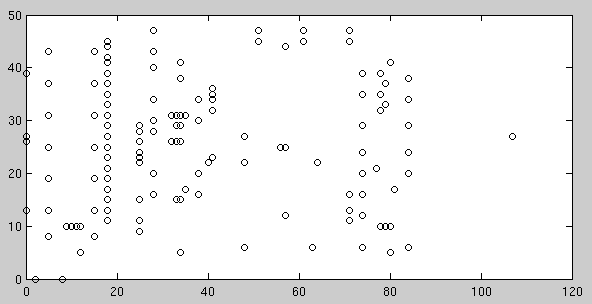
\includegraphics[width=0.32\textwidth]{xqf131}} 

\subfloat[\dataset{xql662} (2513)]{\label{fig:xql662}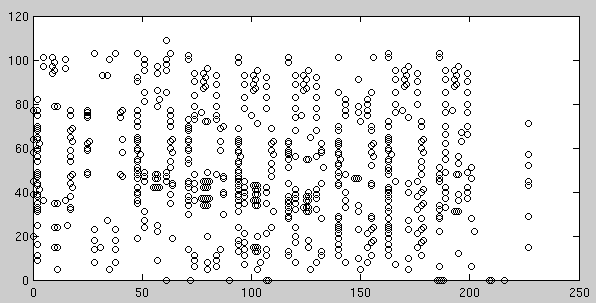
\includegraphics[width=0.32\textwidth]{xql662}} \vspace{0.5cm}
\subfloat[\dataset{rbx711} (3115)]{\label{fig:rbx711}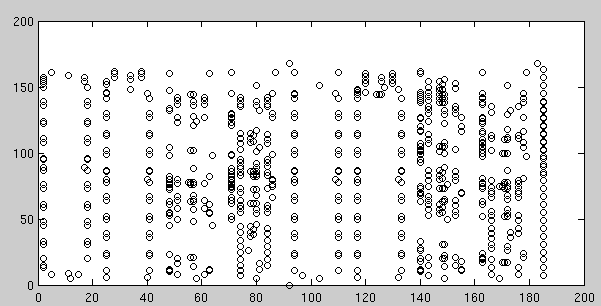
\includegraphics[width=0.32\textwidth]{rbx711}} 
\caption[The five benchmark problems.]{The five benchmark problems. In parentheses their optimal solutions are given.}
\label{fig:datasets}
\end{figure}

The following experiments will therefore be based on 5 benchmark problems, shown in \autoref{fig:datasets}. In particular, these problems consist of respectively 131, 380, 662 and 711 nodes, and one with 41 nodes based on Belgium's most important cities. For all of these except for \dataset{belgiumtour}, we know the optimal solution.
% \begin{table}[hbpt]
% \centering 
% \begin{tabular} {l r}
% \toprule
% name & optimal solution \\ \midrule
% \dataset{belgiumtour}  & ?\\
% \dataset{xqf131}  & 564\\
% \dataset{bcl380}  & 1621\\
% \dataset{xql662}  & 2513\\
% \dataset{rbx711}  & 3115\\\bottomrule
% \end{tabular}
% \caption{Benchmark problems and their characteristics.\label{tab:best}}
% \end{table}


%  


\section{Experiments}
% The implementation of the genetic algorithm is not done from scratch, but is based on an existing \textsc{Matlab} GA toolbox accompanied with a graphical user interface and other functionalities relevant to the TSP problem.
% 
In this section, we will perform experiments to analyze the properties of the various operators for the genetic algorithms with respect to the TSP problem. First, we will investigate the crossover operators, followed by the mutation operators and finally the selection operators.


We will measure the performance by running the genetic algorithm several times for each of the 5 benchmark problems. To be precise, we will run the algorithm 5 times for each problem, and record the computation time and solution quality of each run.  By repeatedly solving different problems, we will also get a measure of how much the applied operators depend on the problem size. And, because benchmark problems have been used, we can also express the quality of the best solution in a relative manner with respect to the global optimum solution. As a measure for this, we use the relative error, i.e., $\epsilon_\textnormal{rel} = \frac{|x_\textnormal{opt} - \hat{x}|}{x_\textnormal{opt}}$.

All experiments were executed with \textsc{Matlab} version 2010b (Linux 64 bit version) on a laptop with an Intel Core i3-370M 2.4\,Ghz and 4\,GB RAM.

\subsection{Crossover operators}
\begin{sidewaystable}[hbpt]\centering
\footnotesize{
\begin{tabular} {l l S  l l S l l S l l S l l S l}
\toprule
&& \multicolumn{2}{c}{\dataset{belgiumtour}} && \multicolumn{2}{c}{\dataset{xqf131}} && \multicolumn{2}{c}{\dataset{bcl380}}  & &\multicolumn{2}{c}{\dataset{xql662}} && \multicolumn{2}{c}{\dataset{rbx711}} \\  \cmidrule{3-4} \cmidrule{6-7} \cmidrule{9-10} \cmidrule{12-13}   \cmidrule{15-16}  
Run & & {Time (s)} & Distance & & {Time (s)} & Distance && {Time (s)} & Distance && {Time (s)} & Distance && {Time (s)} & Distance \\ \midrule\addlinespace
\textbf{AEX}\\
1   &&  24.0 & 1486 && 32.3 & 3250  && 69.5 & 21046  && 110.0 & 45983 && 111.3 & 56082 \\
2   &&  23.6 & 1682 && 33.3 & 3267  && 71.5 & 21223 && 111.2 & 45244 && 120.1 & 56562   \\
3   &&  24.3 & 1498 && 32.2 & 3250 &&  69.5 & 21046 && 116.6 & 45952 && 113.3 & 56522    \\
4   &&  23,7 & 1635&& 31.9 & 3338  && 68.8 & 21757 && 105.9 & 46538 && 114.5 & 56538 \\
5   &&  23.6 & 1519 &&  32.3 & 3380  && 70.3 & 21781 && 107.3 & 46732 && 119.1 & 55268  \\ \addlinespace
Worst  &&  24.3 & 1682 (?) && 33.3 & 3380 (5.0) && 71.4 & 21781 (12.4) && 116.6 & 46732 (18.0) && 120.1 & 56562 (17.2)  \\
Average&&  23.8 & 1564 (?) && 32.4 & 3297 (4.8) && 69.9 & 21371 (12.2) && 110.2 & 46090 (17.3) && 115.7 & 56194 (17.0)    \\
Best   && 23.6 & 1486 (?) && 31.9 & 3250 (4.7)  && 68.8 & 21046 (12.0) && 105.9 & 45244  (17.0)&& 111.3 & 55268 (16.7)     \\\midrule\addlinespace\addlinespace
\textbf{PMX}\\
1   &&  7.0 & 1090 && 8.7 & 2462  &&  16.0 & 18317  && 30.6 & 39367 && 35.2 & 48260 \\
2   &&  7.1 & 1226 && 8.7 & 2242  && 16.5 & 18581 && 31.3 & 39728 &&   34.2 & 50096    \\
3   &&  7.0 & 984 && 8.6 & 2535 &&  16.6 & 18315 &&  32.1    & 40302  && 35.1   & 50821      \\
4   &&  7.1 & 1238 && 8.5 & 2404  && 16.6     &  18373   && 32.7  & 41374 && 33.3  & 50139   \\
5   &&  7.2 & 910 && 8.6 & 2232  && 16.7 &  18244    && 29.6 & 39863  &&  33.5    & 49296    \\ \addlinespace
Worst  &&  7.2 & 1238 (?) && 8.7 & 2535 (3.5) && 16.7  & 18581 (10.5) &&  32.7   & 41374  (15.5) &&  35.2  & 50821 (15.3)  \\
Average&&  7.1 & 1090 (?) && 8.6 & 2375 (3.2) &&  16.5  &  18366 (10.3) &&  32.3 & 40127 (15.0) && 34.3  & 49722 (15.0)    \\
Best   && 7.0 & 910 (?) && 8.5 & 2232 (3.0)  &&  16.0  &  18244 (10.2) &&  29.6 & 39367 (14.7) && 33.3  &  48260 (14.5)     
\\\midrule\addlinespace\addlinespace
\textbf{OX1}\\
1   &&  6.8 & 952 && 8.3 & 2332  && 7.8 & 17290  && 8.3 & 38775 && 8.5 & 48131 \\
2   &&  6.8 & 931 && 7.1 & 2314  && 7.9 & 16928 && 8.2 & 39335 && 8.6 & 48709   \\
3   &&  6.8 & 1002 && 7.0 & 2389 &&  7.7 & 17081 && 8.3 & 39317 && 8.7 & 47980    \\
4   &&  6.8 & 985 && 7.0 & 2309  && 7.8 & 17066 && 8.4 & 38891 && 8.7 & 48180 \\
5   &&  6.9 & 928 &&  7.0 & 2186  && 7.8 & 16670 && 8.3 & 38486 && 8.6 & 48918  \\ \addlinespace
Worst  &&  6.9 & 1002 (?) && 8.3 & 2389 (3.2) && 7.9 & 17290 (10.1) && 8.4 & 39335 (14.7) && 8.7 & 48918 (14.7)  \\
Average&&  6.8& 959 (?) && 7.3 & 2306 (3.1) && 7.8 & 17007 (9.5) && 8.3 & 38960 (14.5) && 8.6 & 48384 (14.5)    \\
Best   && 6.8 & 928 (?) && 7.0 & 2186 (2.9)  && 7.7 & 16670 (9.3)&& 8.2 & 38486 (14.3) && 8.5 & 47980 (14.4)     \\
\bottomrule
\end{tabular}}
\caption[TSP performance on benchmark problems of crossover operators (1).]{TSP performance on benchmark problems of crossover operators: \emph{alternating edge crossover} (AEX), \emph{partially matched crossover} (PMX) and \emph{order crossover} (OX1).}
\label{tab:crossover}
\end{sidewaystable}



\begin{sidewaystable}[hbpt]\centering
\footnotesize{
\begin{tabular} {l l S  l l S l l S l l S l l S l}
\toprule
&& \multicolumn{2}{c}{\dataset{belgiumtour}} && \multicolumn{2}{c}{\dataset{xqf131}} && \multicolumn{2}{c}{\dataset{bcl380}}  & &\multicolumn{2}{c}{\dataset{xql662}} && \multicolumn{2}{c}{\dataset{rbx711}} \\  \cmidrule{3-4} \cmidrule{6-7} \cmidrule{9-10} \cmidrule{12-13}   \cmidrule{15-16}  
Run & & {Time (s)} & Distance & & {Time (s)} & Distance && {Time (s)} & Distance && {Time (s)} & Distance && {Time (s)} & Distance \\ \midrule\addlinespace
\textbf{CX}\\
1   &&  6.6 & 1381 && 6.9 & 3032  && 8.0 & 21334  && 9.6 & 44788 && 9.3 & 56008 \\
2   &&  6.7 & 1223 && 7.1 & 2847  && 8.2 & 21104 && 10.3 & 43846 && 10.2 & 53786  \\
3   &&  6.6 & 1244 && 7.0 & 2828 &&  8.4 & 20150 && 10.0 & 44187 && 10.2 & 55655    \\
4   &&  6.8 & 1354 && 7.0 & 2965  && 8.2 & 20936 && 9.5 & 46068 && 10.9 & 55655 \\
5   &&  6.6 & 1195 &&  7.0 & 2858  && 8.6 & 20274 && 10.6 & 43828 && 9.3 & 55974  \\ \addlinespace
Worst  &&  6.8 & 1381 (?) && 7.1 & 3032 (4.4) && 8.6 & 21334 (12.2) && 10.6 & 46068 (17.3) && 10.9 & 56008 (17.0)  \\
Average&&  6.7 & 1279 (?) && 7.0 & 2906 (4.2) && 8.2 & 20759 (11.8) && 10.0 & 44543 (16.7) && 10.0 & 55472 (16.8)    \\
Best   && 6.6 & 1195 (?) && 6.9 & 2828 (4.0)  && 8.0 & 20150 (11.4)&& 9.5 & 43828 (16.4) && 9.3 & 53786 (16.3)    \\\midrule\addlinespace\addlinespace
\textbf{ERX}\\
1   &&  9.9 & 889 && 18.4 & 1824  &&  119.3 & 13298  && 272.8 & 23010 && 288.0 & 33963 \\
2   &&  10.0 & 926 && 18.8 & 1537  && 118.7 & 14512 && 277.7 & 22584 &&   289.0 & 34295    \\
3   &&  9.9 & 1021 && 18.9 & 1716 &&  120.4 & 13190 &&  264.3    & 22552  && 288.8   & 32114      \\
4   &&  10.6 & 971 && 18.7 & 1619  && 110.0     &  14352       && 269.4  & 23115 && 289.7  & 34034   \\
5   &&  10.0 & 979 && 18.8 & 1666  && 108.9       &  14826    && 265.3  & 22918  &&  290.6    & 33003    \\ \addlinespace
Worst  &&  10.6 & 1021 (?) && 18.9 & 1824 (2.2) && 120.4  & 14826 (8.1) &&  277.7  & 23115 (8.2) &&  290.6  & 34295 (10.0)  \\
Average&&  10.1 & 957 (?) && 18.7 & 1683 (2.0) &&  115.5  &  14036 (7.7) &&  269.9  & 22836 (8.1) && 289.2  & 33482 (9.7)    \\
Best   && 9.9 & 889 (?) && 18.4 & 1573 (1.8)  &&  108.9  &  13190 (7.1)&&  264.3 & 22552 (8.0) && 288.0  &  32114 (9.3)     
\\\midrule\addlinespace\addlinespace
\textbf{EERX}\\
1   &&  10.9 & 892 && 22.0 & 1619  &&  115.7 & 13947  && 267.7 & 24128 && 308.0 & 34244 \\
2   &&  10.7 & 946 && 21.4 & 1699  && 118.8 & 12968 && 281.7 & 24498 &&  291.0 & 33877   \\
3   &&  10.8 & 964 && 22.0 & 1780 &&  119.8 & 13688 &&  253.8    & 25435  && 286.0  & 34136     \\
4   &&  11.0 & 901 && 21.2 & 1780  && 109.3     & 13049   && 257.0 & 24897  && 289.0 & 33511  \\
5   &&  10.8 & 896 && 22.2 & 1613  && 111.4     & 13516       && 252.8  & 24617 && 293.3    & 33780   \\ \addlinespace
Worst  &&  11.0 & 964 (?) && 22.2 & 1824 (2.2) &&  119.8  & 13947  (7.6) && 281.7   & 25435 (9.1) &&  308.0 &  34244 (10.0)  \\
Average&&  10.8 & 920 (?) && 21.8 & 1683 (2.0) && 115.0  & 13443  (7.3) && 262.6   &  24715 (8.8) && 293.5   & 33910  (9.9)    \\
Best   && 10.7 & 892 (?) && 21.2 & 1573 (1.8)  &&  109.3 & 12968  (7.0)&&  252.8 &  24128 (8.6) &&  286.0 &  33511 (9.7)     \\
\bottomrule
\end{tabular}}
\caption[TSP performance on benchmark problems of crossover operators (2).]{TSP performance on benchmark problems of crossover operators: \emph{cyclic crossover} (CX), \emph{edge recombination crossover} (ERX) and \emph{enhanced edge recombination crossover} (EERX).}
\label{tab:crossover2}
\end{sidewaystable}

The parameters for the experiments concerning the crossover operators are as follows. Crossover operator with 90\% probability, simply inversion mutation with 10\% probability, 5\% elitism, stochastic uniform sampling for selection and no further applied heuristics. 
The number of individuals in each generation is 50, and the algorithm is stopped after 100 generations. 
(The crossover probability is set high so that the outcome of the algorithm is very much characterized by the respective applied crossover operator.)


The results of the alternating edge crossover, partially matched crossover and order crossover operators are given in \autoref{tab:crossover}, and of the cycle crossover, edge recombination crossover and its enhanced variant in \autoref{tab:crossover2}.
(The implementation of these crossover operators is found in Appendix~\ref{appendix:crossover} on \autopageref{appendix:crossover}.)
\subsubsection{Alternating edge crossover}
\paragraph{Description}
The alternating edge crossover chooses an edge from the first
parent at random. Then, the partial tour created in this way is extended
with the appropriate edge of the second parent. This partial tour is
extended by the adequate edge of the first parent, etc.

%Performance comparison with others is not possible yet, but several remarks can already be made. For example,
\paragraph{Results}
It can be seen that the computation time does not increase linearly with the problem size.  The solutions drift away from the optimal solution as the problem size increases, because the amount of generations allowed becomes too limited to give good results. 
% \begin{sidewaystable}[hbpt]\centering
\footnotesize{
\begin{tabular} {l l S  l l S l l S l l S l l S l}
\toprule
&& \multicolumn{2}{c}{\dataset{belgiumtour}} && \multicolumn{2}{c}{\dataset{xqf131}} && \multicolumn{2}{c}{\dataset{bcl380}}  & &\multicolumn{2}{c}{\dataset{xql662}} && \multicolumn{2}{c}{\dataset{rbx711}} \\  \cmidrule{3-4} \cmidrule{6-7} \cmidrule{9-10} \cmidrule{12-13}   \cmidrule{15-16}  
Run & & {Time (s)} & Distance & & {Time (s)} & Distance && {Time (s)} & Distance && {Time (s)} & Distance && {Time (s)} & Distance \\ \midrule
1   &&  24.0 & 1486 && 32.3 & 3250  && 69.5 & 21046  && 110.0 & 45983 && 111.3 & 56082 \\
2   &&  23.6 & 1682 && 33.3 & 3267  && 71.5 & 21223 && 111.2 & 45244 && 120.1 & 56562   \\
3   &&  24.3 & 1498 && 32.2 & 3250 &&  69.5 & 21046 && 116.6 & 45952 && 113.3 & 56522    \\
4   &&  23,7 & 1635&& 31.9 & 3338  && 68.8 & 21757 && 105.9 & 46538 && 114.5 & 56538 \\
5   &&  23.6 & 1519 &&  32.3 & 3380  && 70.3 & 21781 && 107.3 & 46732 && 119.1 & 55268  \\ \midrule\addlinespace
Worst  &&  24.3 & 1682 (?) && 33.3 & 3380 (5.0) && 71.4 & 21781 (12.4) && 116.6 & 46732 (18.0) && 120.1 & 56562 (17.2)  \\
Average&&  23.8 & 1564 (?) && 32.4 & 3297 (4.8) && 69.9 & 21371 (12.2) && 110.2 & 46090 (17.3) && 115.7 & 56194 (17.0)    \\
Best   && 23.6 & 1486 (?) && 31.9 & 3250 (4.7)  && 68.8 & 21046 (12.0) && 105.9 & 45244  (17.0)&& 111.3 & 55268 (16.7)     \\
\bottomrule
\end{tabular}}
\caption{TSP performance of adjacency representation with alternating edges crossover (simple inversion mutation).}
\label{tab:adj_performance}
\end{sidewaystable}

We conclude that both the solving time and solution quality of this crossover operator are of very poor quality (as will be seen when compared to the other crossover operators). This is because the alternating edges crossover often destroys good subtours. 




\subsubsection{Partially matched crossover}
\paragraph{Description}
The partially matched crossover (PMX) operator passes on ordering and value information
from the parent tours to the offspring tours: A part of one parent's string
is mapped onto a part of the other parent's string and the remaining
information is exchanged.

% The results of the PMX operator are given in \autoref{tab:pmx_performance}. 
\paragraph{Results}
We already see that this operator consistently gives better results than the alternating edge crossover operator. For computation time, we see a speedup with a factor of $\approxeq 4$; the solution quality is slightly better with roughly 20\%. We see the same issues with the scalability of the TSP sizes as before, only the solution time dependence on the problem size is much smaller in this case. 

The PMX operator therefore tries to keep the positions of the cities in
the path representation; these are rather irrelevant in the context of the
TSP problem where the most important goal is to keep the sequences.
Thus, the performance of this operator for the TSP is rather poor, as shown by the solution quality on the benchmark problems.


% \begin{sidewaystable}[hbpt]\centering
\footnotesize{
\begin{tabular} {l l S  l l S l l S l l S l l S l}
\toprule
&& \multicolumn{2}{c}{\dataset{belgiumtour}} && \multicolumn{2}{c}{\dataset{xqf131}} && \multicolumn{2}{c}{\dataset{bcl380}}  & & \multicolumn{2}{c}{\dataset{xql662}} && \multicolumn{2}{c}{\dataset{rbx711}} \\  \cmidrule{3-4} \cmidrule{6-7} \cmidrule{9-10} \cmidrule{12-13}   \cmidrule{15-16}  
Run & & {Time (s)} & Distance & & {Time (s)} & Distance && {Time (s)} & Distance && {Time (s)} & Distance && {Time (s)} & Distance \\ \midrule
1   &&  7.0 & 1090 && 8.7 & 2462  &&  16.0 & 18317  && 30.6 & 39367 && 35.2 & 48260 \\
2   &&  7.1 & 1226 && 8.7 & 2242  && 16.5 & 18581 && 31.3 & 39728 &&   34.2 & 50096    \\
3   &&  7.0 & 984 && 8.6 & 2535 &&  16.6 & 18315 &&  32.1    & 40302  && 35.1   & 50821      \\
4   &&  7.1 & 1238 && 8.5 & 2404  && 16.6     &  18373   && 32.7  & 41374 && 33.3  & 50139   \\
5   &&  7.2 & 910 && 8.6 & 2232  && 16.7 &  18244    && 29.6 & 39863  &&  33.5    & 49296    \\ \midrule\addlinespace
Worst  &&  7.2 & 1238 (?) && 8.7 & 2535 (3.5) && 16.7  & 18581 (10.5) &&  32.7   & 41374  (15.5) &&  35.2  & 50821 (15.3)  \\
Average&&  7.1 & 1090 (?) && 8.6 & 2375 (3.2) &&  16.5  &  18366 (10.3) &&  32.3 & 40127 (15.0) && 34.3  & 49722 (15.0)    \\
Best   && 7.0 & 910 (?) && 8.5 & 2232 (3.0)  &&  16.0  &  18244 (10.2) &&  29.6 & 39367 (14.7) && 33.3  &  48260 (14.5)     \\
\bottomrule
\end{tabular}}
\caption{TSP performance of path representation with PMX crossover (simple inversion mutation). }
\label{tab:pmx_performance}
\end{sidewaystable}
% 
% \dataset{xqf131}  && 564\\
% \dataset{bcl380}  && 1621\\
% \dataset{xql662}  && 2513\\
% \dataset{rbx711}  && 3115\\
% \dataset{belgiumtour}  && ?\\
% 
\subsubsection{Order crossover}
\paragraph{Description}
The order crossover (OX1) operator constructs an offspring by choosing a subtour of one parent preserving
the relative order of the other parent. 


\paragraph{Results}
% The results of the OX1 operator are given in \autoref{tab:ox_performance}. 
The solution quality of OX1 is better than PMX for all benchmark problems. But more importantly, we see that (this particular implementation of) the operator scales very well with the problem size in terms of computational complexity. 

The solution quality is high because it employs the essential property of the path representation, that the order of cities is important and not their position. Its computational complexity is low because the algorithm is very simple. Overall, this is an operator with a good trade-off between solution quality and computational complexity.
% \begin{sidewaystable}[hbpt]\centering
\footnotesize{
\begin{tabular} {l l S  l l S l l S l l S l l S l}
\toprule
&& \multicolumn{2}{c}{\dataset{belgiumtour}} && \multicolumn{2}{c}{\dataset{xqf131}} && \multicolumn{2}{c}{\dataset{bcl380}}  & &\multicolumn{2}{c}{\dataset{xql662}} && \multicolumn{2}{c}{\dataset{rbx711}} \\  \cmidrule{3-4} \cmidrule{6-7} \cmidrule{9-10} \cmidrule{12-13}   \cmidrule{15-16}  
Run & & {Time (s)} & Distance & & {Time (s)} & Distance && {Time (s)} & Distance && {Time (s)} & Distance && {Time (s)} & Distance \\ \midrule
1   &&  6.8 & 952 && 8.3 & 2332  && 7.8 & 17290  && 8.3 & 38775 && 8.5 & 48131 \\
2   &&  6.8 & 931 && 7.1 & 2314  && 7.9 & 16928 && 8.2 & 39335 && 8.6 & 48709   \\
3   &&  6.8 & 1002 && 7.0 & 2389 &&  7.7 & 17081 && 8.3 & 39317 && 8.7 & 47980    \\
4   &&  6.8 & 985 && 7.0 & 2309  && 7.8 & 17066 && 8.4 & 38891 && 8.7 & 48180 \\
5   &&  6.9 & 928 &&  7.0 & 2186  && 7.8 & 16670 && 8.3 & 38486 && 8.6 & 48918  \\ \midrule\addlinespace
Worst  &&  6.9 & 1002 (?) && 8.3 & 2389 (3.2) && 7.9 & 17290 (10.1) && 8.4 & 39335 (14.7) && 8.7 & 48918 (14.7)  \\
Average&&  6.8& 959 (?) && 7.3 & 2306 (3.1) && 7.8 & 17007 (9.5) && 8.3 & 38960 (14.5) && 8.6 & 48384 (14.5)    \\
Best   && 6.8 & 928 (?) && 7.0 & 2186 (2.9)  && 7.7 & 16670 (9.3)&& 8.2 & 38486 (14.3) && 8.5 & 47980 (14.4)     \\
\bottomrule
\end{tabular}}
\caption{TSP performance of path representation with OX1 crossover (and simple inversion mutation). }
\label{tab:ox_performance}
\end{sidewaystable}
% 
% \dataset{xqf131}  && 564\\
% \dataset{bcl380}  && 1621\\
% \dataset{xql662}  && 2513\\
% \dataset{rbx711}  && 3115\\
% \dataset{belgiumtour}  && ?\\

\subsubsection{Cycle crossover}

\paragraph{Description}
The cyclic crossover (CX) operator attempts to create an offspring from the parents where every position is
occupied by a corresponding element from one of the parents.

% The results of the CX operator are given in \autoref{tab:cx_performance}.

\paragraph{Results}
This operator is somewhat slower than the order crossover and the solution quality is worse than PMX (but still better than AEX). This operator is thus not really interesting because it performs mediocre without any benefits.

In \cite{Oliver}, it was concluded from theoretical and empirical results
that the CX operator gave slightly better results than the PMX operator. 
In our experiments we did not see this result.

However our basic assumption that in the context of the TSP it is much more
important to keep sequences rather than positions, is fortified, as we see that OX is definitely better than PMX and CX.

% \begin{sidewaystable}[hbpt]\centering
\footnotesize{
\begin{tabular} {l l S  l l S l l S l l S l l S l}
\toprule
&& \multicolumn{2}{c}{\dataset{belgiumtour}} && \multicolumn{2}{c}{\dataset{xqf131}} && \multicolumn{2}{c}{\dataset{bcl380}}  & &\multicolumn{2}{c}{\dataset{xql662}} && \multicolumn{2}{c}{\dataset{rbx711}} \\  \cmidrule{3-4} \cmidrule{6-7} \cmidrule{9-10} \cmidrule{12-13}   \cmidrule{15-16}  
Run & & {Time (s)} & Distance & & {Time (s)} & Distance && {Time (s)} & Distance && {Time (s)} & Distance && {Time (s)} & Distance \\ \midrule
1   &&  6.6 & 1381 && 6.9 & 3032  && 8.0 & 21334  && 9.6 & 44788 && 9.3 & 56008 \\
2   &&  6.7 & 1223 && 7.1 & 2847  && 8.2 & 21104 && 10.3 & 43846 && 10.2 & 53786  \\
3   &&  6.6 & 1244 && 7.0 & 2828 &&  8.4 & 20150 && 10.0 & 44187 && 10.2 & 55655    \\
4   &&  6.8 & 1354 && 7.0 & 2965  && 8.2 & 20936 && 9.5 & 46068 && 10.9 & 55655 \\
5   &&  6.6 & 1195 &&  7.0 & 2858  && 8.6 & 20274 && 10.6 & 43828 && 9.3 & 55974  \\ \midrule\addlinespace
Worst  &&  6.8 & 1381 (?) && 7.1 & 3032 (4.4) && 8.6 & 21334 (12.2) && 10.6 & 46068 (17.3) && 10.9 & 56008 (17.0)  \\
Average&&  6.7 & 1279 (?) && 7.0 & 2906 (4.2) && 8.2 & 20759 (11.8) && 10.0 & 44543 (16.7) && 10.0 & 55472 (16.8)    \\
Best   && 6.6 & 1195 (?) && 6.9 & 2828 (4.0)  && 8.0 & 20150 (11.4)&& 9.5 & 43828 (16.4) && 9.3 & 53786 (16.3)     \\
\bottomrule
\end{tabular}}
\caption{TSP performance of path representation with CX crossover (and simple inversion mutation). }
\label{tab:cx_performance}
\end{sidewaystable}
% 
% \dataset{xqf131}  && 564\\
% \dataset{bcl380}  && 1621\\
% \dataset{xql662}  && 2513\\
% \dataset{rbx711}  && 3115\\
% \dataset{belgiumtour}  && ?\\

\subsubsection{(Enhanced) edge recombination crossover}
\paragraph{Description}
Even if the main aim of the OX operator is to keep the sequence of at
least one parent there are still quite a lot of new edges in the offspring.

The edge recombination operator (ERX) has been designed with the
objective of keeping as many edges defined by the parents as possible.

As common sequences of the parent tours are not taken into account by
the ERX operator an enhancement, the enhanced
edge recombination crossover (EERX) has been proposed.

The EERX additionally gives priority to those edges starting from the
current city which are present in both parents.

\paragraph{Results}

% The results of the ERX operator are given in \autoref{tab:erx_performance} and of the EERX operator in \autoref{tab:eerx_performance}. 
The solution quality of these operators is undoubtly the best. It is clear that by keeping as many edges defined by the parents as possible, these operators give very good solutions, but the drawback is that these operators need a very complex and time consuming procedure.

We can also see the improvement of EERX in solution quality versus ERX by sacrificing a relative small amount of computation time.
% \begin{sidewaystable}[hbpt]\centering
\footnotesize{
\begin{tabular} {l l S  l l S l l S l l S l l S l}
\toprule
&& \multicolumn{2}{c}{\dataset{belgiumtour}} && \multicolumn{2}{c}{\dataset{xqf131}} && \multicolumn{2}{c}{\dataset{bcl380}}  & &\multicolumn{2}{c}{\dataset{xql662}} && \multicolumn{2}{c}{\dataset{rbx711}} \\  \cmidrule{3-4} \cmidrule{6-7} \cmidrule{9-10} \cmidrule{12-13}   \cmidrule{15-16}  
Run & & {Time (s)} & Distance & & {Time (s)} & Distance && {Time (s)} & Distance && {Time (s)} & Distance && {Time (s)} & Distance \\ \midrule
1   &&  9.9 & 889 && 18.4 & 1824  &&  119.3 & 13298  && 272.8 & 23010 && 288.0 & 33963 \\
2   &&  10.0 & 926 && 18.8 & 1537  && 118.7 & 14512 && 277.7 & 22584 &&   289.0 & 34295    \\
3   &&  9.9 & 1021 && 18.9 & 1716 &&  120.4 & 13190 &&  264.3    & 22552  && 288.8   & 32114      \\
4   &&  10.6 & 971 && 18.7 & 1619  && 110.0     &  14352       && 269.4  & 23115 && 289.7  & 34034   \\
5   &&  10.0 & 979 && 18.8 & 1666  && 108.9       &  14826    && 265.3  & 22918  &&  290.6    & 33003    \\ \midrule\addlinespace
Worst  &&  10.6 & 1021 (?) && 18.9 & 1824 (2.2) && 120.4  & 14826 (8.1) &&  277.7  & 23115 (8.2) &&  290.6  & 34295 (10.0)  \\
Average&&  10.1 & 957 (?) && 18.7 & 1683 (2.0) &&  115.5  &  14036 (7.7) &&  269.9  & 22836 (8.1) && 289.2  & 33482 (9.7)    \\
Best   && 9.9 & 889 (?) && 18.4 & 1573 (1.8)  &&  108.9  &  13190 (7.1)&&  264.3 & 22552 (8.0) && 288.0  &  32114 (9.3)     \\
\bottomrule
\end{tabular}}
\caption{TSP performance of path representation with ERX crossover (and simple inversion mutation). }
\label{tab:erx_performance}
\end{sidewaystable}
% 
% \dataset{xqf131}  && 564\\
% \dataset{bcl380}  && 1621\\
% \dataset{xql662}  && 2513\\
% \dataset{rbx711}  && 3115\\
% \dataset{belgiumtour}  && ?\\

% \begin{sidewaystable}[hbpt]\centering
\footnotesize{
\begin{tabular} {l l S  l l S l l S l l S l l S l}
\toprule
&& \multicolumn{2}{c}{\dataset{belgiumtour}} && \multicolumn{2}{c}{\dataset{xqf131}} && \multicolumn{2}{c}{\dataset{bcl380}}  & &\multicolumn{2}{c}{\dataset{xql662}} && \multicolumn{2}{c}{\dataset{rbx711}} \\  \cmidrule{3-4} \cmidrule{6-7} \cmidrule{9-10} \cmidrule{12-13}   \cmidrule{15-16}  
Run & & {Time (s)} & Distance & & {Time (s)} & Distance && {Time (s)} & Distance && {Time (s)} & Distance && {Time (s)} & Distance \\ \midrule
1   &&  10.9 & 892 && 22.0 & 1619  &&  115.7 & 13947  && 267.7 & 24128 && 308.0 & 34244 \\
2   &&  10.7 & 946 && 21.4 & 1699  && 118.8 & 12968 && 281.7 & 24498 &&  291.0 & 33877   \\
3   &&  10.8 & 964 && 22.0 & 1780 &&  119.8 & 13688 &&  253.8    & 25435  && 286.0  & 34136     \\
4   &&  11.0 & 901 && 21.2 & 1780  && 109.3     & 13049   && 257.0 & 24897  && 289.0 & 33511  \\
5   &&  10.8 & 896 && 22.2 & 1613  && 111.4     & 13516       && 252.8  & 24617 && 293.3    & 33780   \\ \midrule\addlinespace
Worst  &&  11.0 & 964 (?) && 22.2 & 1824 (2.2) &&  119.8  & 13947  (7.6) && 281.7   & 25435 (9.1) &&  308.0 &  34244 (10.0)  \\
Average&&  10.8 & 920 (?) && 21.8 & 1683 (2.0) && 115.0  & 13443  (7.3) && 262.6   &  24715 (8.8) && 293.5   & 33910  (9.9)    \\
Best   && 10.7 & 892 (?) && 21.2 & 1573 (1.8)  &&  109.3 & 12968  (7.0)&&  252.8 &  24128 (8.6) &&  286.0 &  33511 (9.7)     \\
\bottomrule
\end{tabular}}
\caption{TSP performance of path representation with EERX crossover (and simple inversion mutation). }
\label{tab:eerx_performance}
\end{sidewaystable}
% 
% \dataset{xqf131}  && 564\\
% \dataset{bcl380}  && 1621\\
% \dataset{xql662}  && 2513\\
% \dataset{rbx711}  && 3115\\
% \dataset{belgiumtour}  && ?\\



% \clearpage
\subsection{Mutation operators}
The parameters for the experiments concerning the mutation operators are as follows. Crossover operator with 10\% probability, mutation operator with 90\% probability, 5\% elitism, stochastic uniform sampling for selection and no further applied heuristics. The number of individuals in each generation is 50, and the algorithm is stopped after 100 generations. 
(The mutation probability is set high so that the outcome of the algorithm is very much characterized by the respective applied mutation operator.)

The results of the simple inversion, inversion, exchange and insertion mutation operators are given in \autoref{tab:mutation}.
(The implementation of these mutation operators is found in Appendix~\ref{appendix:mutation} on \autopageref{appendix:mutation}.)
% 
% We fixed the crossover operator to OX1 and EERX because they gave the most interesting results in terms of time complexity and solution quality as shown in the previous section. We only performed the experiments on \dataset{bcl380} because of time and space constraints. 
% % The results are shown in respectively \autoref{tab:mutation1_performance} and \autoref{tab:mutation2_performance}.

\begin{sidewaystable}[hbpt]\centering
\footnotesize{
\begin{tabular} {l l S  l l S l l S l l S l l S l}
\toprule
&& \multicolumn{2}{c}{\dataset{belgiumtour}} && \multicolumn{2}{c}{\dataset{xqf131}} && \multicolumn{2}{c}{\dataset{bcl380}}  & &\multicolumn{2}{c}{\dataset{xql662}} && \multicolumn{2}{c}{\dataset{rbx711}} \\  \cmidrule{3-4} \cmidrule{6-7} \cmidrule{9-10} \cmidrule{12-13}   \cmidrule{15-16}  
Run & & {Time (s)} & Distance & & {Time (s)} & Distance && {Time (s)} & Distance && {Time (s)} & Distance && {Time (s)} & Distance \\ \midrule\addlinespace
\textbf{simple inversion} \\
1   &&  6.8 & 1090 && 6.8 & 2530  &&  7.5 & 19014  && 8.5 & 41125 && 8.4 & 53679 \\
2   &&  6.7 & 1090 && 6.8 & 2404  && 7.7 & 18897 && 8.0 & 42498 &&  8.8 & 54119   \\
3   &&  6.7 & 1081 && 6.8 & 2496 &&  7.4 & 18592 &&  8.9    & 42802  && 8.5  & 52536     \\
4   &&  6.7 & 1004 && 7.2 & 2444  && 8.6     & 18303   && 9.3 & 42033  && 9.4 & 51366  \\
5   &&  7.3 & 1182 && 7.6 & 2446  && 8.3    & 19469       && 9.1 & 43261 && 9.5   & 53439   \\ \addlinespace
Worst  &&  7.3 & 1182 (?) && 7.6 & 2530 (3.5) &&  8.6  &  19469  (11.0) && 9.3  & 43261 (16.2) &&  9.5 &  54119 (16.4)  \\
Average&&  6.8 & 1089 (?) && 7.0 & 2464 (3.4) && 7.9  & 18856  (10.6) && 8.8   &  42424 (15.9) && 8.9  &  53028 (16.0)    \\
Best   && 6.7 & 1004 (?) && 6.8 & 2404 (3.3)  &&  7.4 & 18303  (10.3) &&  8.0 &  41125 (15.3) &&  8.4 &  51366 (15.5)     \\\midrule\addlinespace\addlinespace
\textbf{inversion} \\
1   &&  7.0 & 1144 && 7.1 & 2454  &&  8.6 & 18562  && 9.2 & 42705 && 9.6 & 51351 \\
2   &&  7.1 & 1200 && 7.0 & 2460  && 8.7 & 18396 && 9.0 & 42384 &&  9.2 & 52843   \\
3   &&  6.9 & 1378 && 7.0 & 2523 &&  8.3 & 18950 &&  9.9   & 40665  && 9.5  & 52511     \\
4   &&  7.1 & 1230 && 7.6 & 2484  && 8.7     & 18402   && 8.9 & 41613  && 9.4 & 51824  \\
5   &&  7.7 & 1265 && 7.5 & 2434  && 8.1   & 18975       && 9.0 & 42298 && 9.3   &  52342  \\ \addlinespace
Worst  &&  7.7 & 1378 (?) && 7.6 & 2523 (3.5) &&  8.7  &  18975  (10.7) && 9.9  & 42705 (16.0) &&  9.6 &  52843 (16.0)  \\
Average&&  7.2 & 1243 (?) && 7.2 & 2471 (3.4) &&8.5  & 18657  (10.5) && 9.2  &  41933 (15.7) && 9.4 &  52174 (15.7)    \\
Best   && 6.9 & 1144 (?) && 7.0 & 2434 (3.3)  &&  8.1 & 18396  (10.3) &&  8.9 &  40665 (15.2) &&  9.2 &  51351 (15.5)    \\\midrule\addlinespace\addlinespace
\textbf{insertion} \\
1   &&  7.2 & 1254 && 7.2 & 2689  &&  8.6 & 19387  && 9.2 & 42436 && 9.5 & 52299 \\
2   &&  7.2 & 1163 && 7.3 & 2778  && 8.0 & 18499 && 8.9 & 42602 &&  9.1 & 52499   \\
3   &&  7.0 & 1265 && 7.4 & 2483 &&  7.6 & 19252 &&  8.9   & 42040  && 8.8  & 53086     \\
4   &&  7.2 & 1260 && 7.1 & 2558  && 8.3     & 19212   && 8.9 & 43277  && 9.4 & 52389  \\
5   &&  7.3 & 1081 && 7.3 & 2512  && 8.2   & 18510       && 9.0 & 43329 && 9.1   &  53047  \\ \addlinespace
Worst  &&  7.3 & 1265 (?) && 7.4 & 2778 (3.9) &&  8.6  &  19252  (10.9) && 9.2  & 43329 (16.0) &&  9.5 &  53086 (16.0)  \\
Average&&  7.2 & 1205 (?) && 7.3 & 2604 (3.6) && 8.1  & 18972  (10.7) && 9.0  &  42737 (16.0) && 9.2 &  52664 (15.9)    \\
Best   && 7.0 & 1081 (?) && 7.1 & 2483 (3.4)  &&  7.6 & 18499  (10.4)&&  8.9 &  42040 (15.7) &&  8.8 &  52299 (15.8)     
\\\midrule\addlinespace\addlinespace
\textbf{exchange} \\
1   &&  7.5 & 1274 && 7.2 & 2742  &&  8.5 & 18994  && 9.4 & 42085 && 9.4 & 52763 \\
2   &&  7.6 & 1212 && 7.3 & 2706  && 7.9 & 18645 && 8.7 & 41072 &&  9.4 & 50406   \\
3   &&  7.0 & 1241 && 7.4 & 2619 &&  8.2 & 18570 &&  8.8   & 41692  &&  9.4  & 52166     \\
4   &&  7.2 & 1205 && 7.1 & 2624  && 8.2     & 19286   && 8.8 & 42493  && 9.2 & 51147  \\
5   &&  7.2 & 1269 && 7.3 & 2782  && 7.9  & 18601      && 9.0 & 41614 && 9.2   &  52047  \\ \addlinespace
Worst  && 7.6  & 1274 (?) && 7.4 & 2782 (3.9) &&  8.5  &  19286  (10.9) && 9.4  & 42493 (15.9) &&  9.4 &  52763 (15.9)  \\
Average&&  7.3 & 1240 (?) && 7.3 & 2695 (3.8) && 8.1 & 18819  (10.6) &&  8.9 &   41791 (15.6) && 9.3 &  51706 (15.8)    \\
Best   && 7.0 & 1205 (?) && 7.1 & 2619 (3.6)  &&  7.9 & 18570  (10.5)&&  8.8 &  41072 (15.3) &&  9.2 &  50406 (15.2) \\    
\bottomrule
\end{tabular}}
\caption[TSP performance on benchmark problems of mutation operators.]{TSP performance on benchmark problems of mutation operators: \emph{simple inversion}, \emph{inversion}, \emph{insertion} and \emph{exchange}.}
\label{tab:mutation}
\end{sidewaystable}















% \begin{sidewaystable}[hbpt]\centering
% \footnotesize{
% \begin{tabular} {ll Sl l Sl l Sl l Sl }
% \toprule
% && \multicolumn{2}{c}{simple inversion} && \multicolumn{2}{c}{inversion} && \multicolumn{2}{c}{exchange}  & & \multicolumn{2}{c}{insertion} \\  \cmidrule{3-4} \cmidrule{6-7} \cmidrule{9-10} \cmidrule{12-13}  
% Run & & {Time (s)} & Distance & & {Time (s)} & Distance && {Time (s)} & Distance && {Time (s)} & Distance  \\ \midrule
% 1   &&  8.4 & 17311 &&  8.9 & 17281  && 8.9  &  17955 && 8.8   & 17656 \\
% 2   &&  8.7 & 17539 && 8.5 & 17691  &&  8.8 & 17701 &&  8.6   &  17150 \\
% 3   &&  8.9 & 17259 && 8.8 & 16836 && 8.8  & 16596 &&   8.7   &  17396       \\
% 4   &&  8.8 & 17565 && 8.8 & 17896   &&  8.8     & 16914    &&  8.7   &  17726   \\
% 5   &&  8.8 & 17801 && 8.7   & 17530  && 8.7 &  16910    &&    8.6       &  17581   \\ \midrule\addlinespace
% Worst  &&  8.9 &  17801 (10.0) && 8.9  & 17896 (10.0) && 8.9 & 17896 (10.0) && 8.8     & 17726 (9.9)   \\
% Average&& 8.7  &  17495 (9.8) && 8.7 &  17447 (9.8) &&  8.8  &   17215 (9.6) && 8.7  & 17502 (9.8)     \\
% Best   &&    8.4 & 17259  (9.6) && 8.5 & 16386 (9.4)  && 8.7    & 16596 (9.2) && 8.6   &  17150 (9.6)    \\
% \bottomrule
% \end{tabular}}
% \caption{TSP performance of mutation operators for path representation with OX on \dataset{bcl380}.}
% \label{tab:mutation1_performance}
% \end{sidewaystable}
% 
% 
% 
% \begin{sidewaystable}[hbpt]\centering
% \footnotesize{
% \begin{tabular} {ll Sl l Sl l Sl l Sl }
% \toprule
% && \multicolumn{2}{c}{simple inversion} && \multicolumn{2}{c}{inversion} && \multicolumn{2}{c}{exchange}  & & \multicolumn{2}{c}{insertion} \\  \cmidrule{3-4} \cmidrule{6-7} \cmidrule{9-10} \cmidrule{12-13}  
% Run & & {Time (s)} & Distance & & {Time (s)} & Distance && {Time (s)} & Distance && {Time (s)} & Distance  \\ \midrule
% 1   &&  111.4 & 13915 &&  110.5 & 13836  && 111.4 &  13713 && 110.8  & 14337 \\
% 2   && 110.6 & 13283 && 111.7 & 13123  && 118.2 & 13826 &&  111.2  &  15050 \\
% 3   && 110.3 & 13098 && 111.2 & 13062 && 112.2  & 14389 &&   108.2  &  14282       \\
% 4   &&  110.5 & 14019 && 110.3 & 13127   &&  113.2     & 14643    &&  109.0   &  13664   \\
% 5   &&  108.3 & 13750 && 109.5   & 13668  && 110.3&  13630    &&    109.9      &  14021   \\ \midrule\addlinespace
% Worst  &&  111.4 &  14019 (7.6) &&  111.7 & 13836 (7.5) && 118.2    & 14643 (8.0) &&  111.2    &  15050 (8.3)   \\
% Average&& 110.2  &  13613 (7.4) && 110.6 &  13636 (7.4) && 113.1   &  14050 (7.7) && 109.8 & 14271 (7.8)     \\
% Best   &&    108.3 & 13098 (7.1) && 109.5 &  13062  (7.1)  && 110.3    &  13630 (7.4) && 108.2   & 13664  (7.4)    \\
% \bottomrule
% \end{tabular}}
% \caption{TSP performance of mutation operators for path representation with EERX on \dataset{bcl380}.}
% \label{tab:mutation2_performance}
% \end{sidewaystable}










%%%%%%%%%
% 
% \begin{sidewaystable}[hbpt]\centering
% \footnotesize{
% \begin{tabular} {ll Sl l Sl l Sl l Sl }
% \toprule
% && \multicolumn{2}{c}{simple inversion} && \multicolumn{2}{c}{inversion} && \multicolumn{2}{c}{exchange}  & & \multicolumn{2}{c}{insertion} \\  \cmidrule{3-4} \cmidrule{6-7} \cmidrule{9-10} \cmidrule{12-13}  
% Run & & {Time (s)} & Distance & & {Time (s)} & Distance && {Time (s)} & Distance && {Time (s)} & Distance  \\ \midrule
% 1   &&  111.4 & 13915 &&  110.5 & 13836  && 111.4 &  13713 && 110.8  & 14337 \\
% 2   && 110.6 & 13283 && 111.7 & 13123  && 118.2 & 13826 &&  111.2  &  15050 \\
% 3   && 110.3 & 13098 && 111.2 & 13062 && 112.2  & 14389 &&   108.2  &  14282       \\
% 4   &&  110.5 & 14019 && 110.3 & 13127   &&  113.2     & 14643    &&  109.0   &  13664   \\
% 5   &&  108.3 & 13750 && 109.5   & 13668  && 110.3&  13630    &&    109.9      &  14021   \\ \midrule\addlinespace
% Worst  &&  8.9 &  17801 () && 8.9  & 17896 && 8.9 & 17896 () && 8.8     & 17726 ()   \\
% Average&& 8.7  &  17495 () && 8.7 &  17447 () &&  8.8  &   17215 () && 8.7  & 17502 ()     \\
% Best   &&    8.4 & 17259  () && 8.5 & 16386 ()  && 8.7    & 16596   () && 8.6   &  17150 ()    \\
% \bottomrule
% \end{tabular}}
% \caption{TSP performance of path representation with xxx on \dataset{bcl380}. Mutation rate: 35\%.}
% \label{tab:mutation3_performance}
% \end{sidewaystable}



\subsubsection{Simple inversion mutation}
\paragraph{Description}

% The results of the simple inversion operator are given in \autoref{tab:simple_inversion_performance}. 
% \begin{sidewaystable}[hbpt]\centering
\footnotesize{
\begin{tabular} {l l S  l l S l l S l l S l l S l}
\toprule
&& \multicolumn{2}{c}{\dataset{belgiumtour}} && \multicolumn{2}{c}{\dataset{xqf131}} && \multicolumn{2}{c}{\dataset{bcl380}}  & &\multicolumn{2}{c}{\dataset{xql662}} && \multicolumn{2}{c}{\dataset{rbx711}} \\  \cmidrule{3-4} \cmidrule{6-7} \cmidrule{9-10} \cmidrule{12-13}   \cmidrule{15-16}  
Run & & {Time (s)} & Distance & & {Time (s)} & Distance && {Time (s)} & Distance && {Time (s)} & Distance && {Time (s)} & Distance \\ \midrule
1   &&  6.8 & 1090 && 6.8 & 2530  &&  7.5 & 19014  && 8.5 & 41125 && 8.4 & 53679 \\
2   &&  6.7 & 1090 && 6.8 & 2404  && 7.7 & 18897 && 8.0 & 42498 &&  8.8 & 54119   \\
3   &&  6.7 & 1081 && 6.8 & 2496 &&  7.4 & 18592 &&  8.9    & 42802  && 8.5  & 52536     \\
4   &&  6.7 & 1004 && 7.2 & 2444  && 8.6     & 18303   && 9.3 & 42033  && 9.4 & 51366  \\
5   &&  7.3 & 1182 && 7.6 & 2446  && 8.3    & 19469       && 9.1 & 43261 && 9.5   & 53439   \\ \midrule\addlinespace
Worst  &&  7.3 & 1182 (?) && 7.6 & 2530 (3.5) &&  8.6  &  19469  (11.0) && 9.3  & 43261 (16.2) &&  9.5 &  54119 (16.4)  \\
Average&&  6.8 & 1089 (?) && 7.0 & 2464 (3.4) && 7.9  & 18856  (10.6) && 8.8   &  42424 (15.9) && 8.9  &  53028 (16.0)    \\
Best   && 6.7 & 1004 (?) && 6.8 & 2404 (3.3)  &&  7.4 & 18303  (10.3) &&  8.0 &  41125 (15.3) &&  8.4 &  51366 (15.5)     \\
\bottomrule
\end{tabular}}
\caption{TSP performance of path representation with simple inversion mutation (and OX1 crossover). }
\label{tab:simple_inversion_performance}
\end{sidewaystable}
% 
% \dataset{xqf131}  && 564\\
% \dataset{bcl380}  && 1621\\
% \dataset{xql662}  && 2513\\
% \dataset{rbx711}  && 3115\\
% \dataset{belgiumtour}  && ?\\

The simple inversion mutation operator randomly selects two cut points and simply reverses the string between them.

\paragraph{Results}
We cannot yet compare with the other mutation operators, but we can already compare with the results of the OX1 results in \autoref{tab:crossover}, where the same parameters were used except for a higher crossover rate and lower mutation rate.   

The solution distances now are significantly worse. This is a straightforward result, since the differences in implementation of the crossover operators are way more pronounced, and thus affect the efficiency of the search space exploration in a profound manner. The same does not hold for the mutation operators, for which these small differences in implementation do not have a strong effect on the way the search space is exploited. Also, for the crossover operators it is way easier to counteract the building block theory and destroy relevant alleles. Mutation operators only introduce small changes, and do not threaten the genetic building blocks as much.    

\subsubsection{Inversion mutation}
% The results of the inversion operator are given in \autoref{tab:inversion_performance}. 
% \begin{sidewaystable}[hbpt]\centering
\footnotesize{
\begin{tabular} {l l S  l l S l l S l l S l l S l}
\toprule
&& \multicolumn{2}{c}{\dataset{belgiumtour}} && \multicolumn{2}{c}{\dataset{xqf131}} && \multicolumn{2}{c}{\dataset{bcl380}}  & &\multicolumn{2}{c}{\dataset{xql662}} && \multicolumn{2}{c}{\dataset{rbx711}} \\  \cmidrule{3-4} \cmidrule{6-7} \cmidrule{9-10} \cmidrule{12-13}   \cmidrule{15-16}  
Run & & {Time (s)} & Distance & & {Time (s)} & Distance && {Time (s)} & Distance && {Time (s)} & Distance && {Time (s)} & Distance \\ \midrule
1   &&  7.0 & 1144 && 7.1 & 2454  &&  8.6 & 18562  && 9.2 & 42705 && 9.6 & 51351 \\
2   &&  7.1 & 1200 && 7.0 & 2460  && 8.7 & 18396 && 9.0 & 42384 &&  9.2 & 52843   \\
3   &&  6.9 & 1378 && 7.0 & 2523 &&  8.3 & 18950 &&  9.9   & 40665  && 9.5  & 52511     \\
4   &&  7.1 & 1230 && 7.6 & 2484  && 8.7     & 18402   && 8.9 & 41613  && 9.4 & 51824  \\
5   &&  7.7 & 1265 && 7.5 & 2434  && 8.1   & 18975       && 9.0 & 42298 && 9.3   &  52342  \\ \midrule\addlinespace
Worst  &&  7.7 & 1378 (?) && 7.6 & 2523 (3.5) &&  8.7  &  18975  (10.7) && 9.9  & 42705 (16.0) &&  9.6 &  52843 (16.0)  \\
Average&&  7.2 & 1243 (?) && 7.2 & 2471 (3.4) &&8.5  & 18657  (10.5) && 9.2  &  41933 (15.7) && 9.4 &  52174 (15.7)    \\
Best   && 6.9 & 1144 (?) && 7.0 & 2434 (3.3)  &&  8.1 & 18396  (10.3) &&  8.9 &  40665 (15.2) &&  9.2 &  51351 (15.5)     \\
\bottomrule
\end{tabular}}
\caption{TSP performance of path representation with inversion mutation (and OX1 crossover).}
\label{tab:inversion_performance}
\end{sidewaystable}
% 
% \dataset{xqf131}  && 564\\
% \dataset{bcl380}  && 1621\\
% \dataset{xql662}  && 2513\\
% \dataset{rbx711}  && 3115\\
% \dataset{belgiumtour}  && ?\\
\paragraph{Description}
The inversion mutation operator randomly selects a subtour, removes it, and inserts it in reverse order at a randomly chosen position.

\paragraph{Results}
This mutation operator requires slightly more calculation time than the previous operator. This is due to the fact that calculation of one extra random position has to be done and the insertion of the subtour in the result.
For the solution quality, we see no significant differences.




\subsubsection{Insertion mutation}
% The results of the insertion operator are given in \autoref{tab:insertion_performance}. 
% \begin{sidewaystable}[hbpt]\centering
\footnotesize{
\begin{tabular} {l l S  l l S l l S l l S l l S l}
\toprule
&& \multicolumn{2}{c}{\dataset{belgiumtour}} && \multicolumn{2}{c}{\dataset{xqf131}} && \multicolumn{2}{c}{\dataset{bcl380}}  & &\multicolumn{2}{c}{\dataset{xql662}} && \multicolumn{2}{c}{\dataset{rbx711}} \\  \cmidrule{3-4} \cmidrule{6-7} \cmidrule{9-10} \cmidrule{12-13}   \cmidrule{15-16}  
Run & & {Time (s)} & Distance & & {Time (s)} & Distance && {Time (s)} & Distance && {Time (s)} & Distance && {Time (s)} & Distance \\ \midrule
1   &&  7.2 & 1254 && 7.2 & 2689  &&  8.6 & 19387  && 9.2 & 42436 && 9.5 & 52299 \\
2   &&  7.2 & 1163 && 7.3 & 2778  && 8.0 & 18499 && 8.9 & 42602 &&  9.1 & 52499   \\
3   &&  7.0 & 1265 && 7.4 & 2483 &&  7.6 & 19252 &&  8.9   & 42040  && 8.8  & 53086     \\
4   &&  7.2 & 1260 && 7.1 & 2558  && 8.3     & 19212   && 8.9 & 43277  && 9.4 & 52389  \\
5   &&  7.3 & 1081 && 7.3 & 2512  && 8.2   & 18510       && 9.0 & 43329 && 9.1   &  53047  \\ \midrule\addlinespace
Worst  &&  7.3 & 1265 (?) && 7.4 & 2778 (3.9) &&  8.6  &  19252  (10.9) && 9.2  & 43329 (16.0) &&  9.5 &  53086 (16.0)  \\
Average&&  7.2 & 1205 (?) && 7.3 & 2604 (3.6) && 8.1  & 18972  (10.7) && 9.0  &  42737 (16.0) && 9.2 &  52664 (15.9)    \\
Best   && 7.0 & 1081 (?) && 7.1 & 2483 (3.4)  &&  7.6 & 18499  (10.4)&&  8.9 &  42040 (15.7) &&  8.8 &  52299 (15.8)     \\
\bottomrule
\end{tabular}}
\caption{TSP performance of path representation with insertion mutation (and OX1 crossover).}
\label{tab:insertion_performance}
\end{sidewaystable}
% 
% \dataset{xqf131}  && 564\\
% \dataset{bcl380}  && 1621\\
% \dataset{xql662}  && 2513\\
% \dataset{rbx711}  && 3115\\
% \dataset{belgiumtour}  && ?\\
\paragraph{Description}
The insertion mutation operator randomly chooses a city, removes it from the tour and inserts it at a randomly selected place. 



\paragraph{Results}
Also for the insertion mutation, we see no substantial improvements in solution quality. As for the time cost, it is on the same order as the inversion mutation.


\subsubsection{Exchange mutation}
% The results of the exchange operator are given in \autoref{tab:exchange_performance}. 
% \begin{sidewaystable}[hbpt]\centering
\footnotesize{
\begin{tabular} {l l S  l l S l l S l l S l l S l}
\toprule
&& \multicolumn{2}{c}{\dataset{belgiumtour}} && \multicolumn{2}{c}{\dataset{xqf131}} && \multicolumn{2}{c}{\dataset{bcl380}}  & &\multicolumn{2}{c}{\dataset{xql662}} && \multicolumn{2}{c}{\dataset{rbx711}} \\  \cmidrule{3-4} \cmidrule{6-7} \cmidrule{9-10} \cmidrule{12-13}   \cmidrule{15-16}  
Run & & {Time (s)} & Distance & & {Time (s)} & Distance && {Time (s)} & Distance && {Time (s)} & Distance && {Time (s)} & Distance \\ \midrule
1   &&  7.5 & 1274 && 7.2 & 2742  &&  8.5 & 18994  && 9.4 & 42085 && 9.4 & 52763 \\
2   &&  7.6 & 1212 && 7.3 & 2706  && 7.9 & 18645 && 8.7 & 41072 &&  9.4 & 50406   \\
3   &&  7.0 & 1241 && 7.4 & 2619 &&  8.2 & 18570 &&  8.8   & 41692  &&  9.4  & 52166     \\
4   &&  7.2 & 1205 && 7.1 & 2624  && 8.2     & 19286   && 8.8 & 42493  && 9.2 & 51147  \\
5   &&  7.2 & 1269 && 7.3 & 2782  && 7.9  & 18601      && 9.0 & 41614 && 9.2   &  52047  \\ \midrule\addlinespace
Worst  && 7.6  & 1274 (?) && 7.4 & 2782 (3.9) &&  8.5  &  19286  (10.9) && 9.4  & 42493 (15.9) &&  9.4 &  52763 (15.9)  \\
Average&&  7.3 & 1240 (?) && 7.3 & 2695 (3.8) && 8.1 & 18819  (10.6) &&  8.9 &   41791 (15.6) && 9.3 &  51706 (15.8)    \\
Best   && 7.0 & 1205 (?) && 7.1 & 2619 (3.6)  &&  7.9 & 18570  (10.5)&&  8.8 &  41072 (15.3) &&  9.2 &  50406 (15.2)     \\
\bottomrule
\end{tabular}}
\caption{TSP performance of path representation with exchange mutation (and OX1 crossover).}
\label{tab:exchange_performance}
\end{sidewaystable}
% 
% \dataset{xqf131}  && 564\\
% \dataset{bcl380}  && 1621\\
% \dataset{xql662}  && 2513\\
% \dataset{rbx711}  && 3115\\
% \dataset{belgiumtour}  && ?\\
\paragraph{Description}
The exchange mutation operator selects two cities of the tour randomly and simply exchanges them. 


\paragraph{Results}
This operator has the same performance as the insertion and inversion mutation.

% 
% \subsubsection{Overview}
% As mentioned in \autoref{sec:tasks} we discuss following mutation operators \cite{affenzeller2009genetic}:
% \begin{description}
%  \item[Simple inversion] The simple inversion mutation operator randomly selects two cut points and simply reverses the string between them.
%  \item[Inversion] The inversion mutation operator randomly selects a subtour, removes it, and inserts it in reverse order at a randomly chosen position.
%  \item[Exchange] The exchange mutation operator selects two cities of the tour randomly and simply exchanges them. 
%  \item[Insertion] The insertion mutation operator randomly chooses a city, removes it from the tour and inserts it at a randomly selected place. 
% \end{description}


% \subsubsection{Experiments}





% \subsubsection{Results}
% All the mutation operators performed nearly equally: there is no significant difference in terms of solution quality nor time complexity, neither in combination with OX or EERX crossover. In terms of ease of implementation, one could argue that the exchange mutation is the easiest, followed by insertion and then simple inversion and inversion. However \textsc{Matlab} makes all these mutation operators very easy and efficient to implement. 
% 
% So in conclusion, the choice of the mutation operator is much less important than the crossover operator for the TSP problem.



\subsection{Selection operators}

The selection operators implemented are stochastic uniform sampling, which was already given in the toolbox and used, a roulette wheel selection (which was also part of the toolbox) and a tournament selection. %All of these are parent selection operators. 
%Nog een klein beetje uitleg over selective pressure, genetische diversiteit, hoe de %elite omhoogdoen voor snelle premature convergence kan zorgen).
For the experiments we use OX1 crossover with 90\% probability, simple inversion mutation with 10\% probability, and 20\% elitism, and 100 consecutive generations with 50 individuals each. No extra heuristics were applied.  

The results of all selection operators are given in \autoref{tab:sus}. (The implementation of these selection operators is found in Appendix~\ref{appendix:selection} on \autopageref{appendix:selection}.)
\subsubsection{Stochastic uniform sampling}
\paragraph{Description}
The stochastic uniform sampling is the parent selection technique that was already given in the \textsc{Matlab} toolbox and originally used. 
This sampling technique provides zero bias and minimum spread. The individuals are mapped to contiguous segments of a line, such that each individual's segment is equal in size to its fitness exactly as in roulette-wheel selection (see further). Here equally spaced pointers are placed over the line as many as there are individuals to be selected.

\begin{sidewaystable}[hbpt]\centering
\footnotesize{
\begin{tabular} {l l S  l l S l l S l l S l l S l}
\toprule
&& \multicolumn{2}{c}{\dataset{belgiumtour}} && \multicolumn{2}{c}{\dataset{xqf131}} && \multicolumn{2}{c}{\dataset{bcl380}}  & &\multicolumn{2}{c}{\dataset{xql662}} && \multicolumn{2}{c}{\dataset{rbx711}} \\  \cmidrule{3-4} \cmidrule{6-7} \cmidrule{9-10} \cmidrule{12-13}   \cmidrule{15-16}  
Run & & {Time (s)} & Distance & & {Time (s)} & Distance && {Time (s)} & Distance && {Time (s)} & Distance && {Time (s)} & Distance \\ \midrule\addlinespace
\textbf{SUS} \\
1   &&  7.2 & 951 && 7.3 & 2268  && 8.1 & 17675  && 8.7 & 39012 && 8.7 & 47856 \\
2   &&  7.1 & 1048 && 7.3 & 2357  && 8.1 & 17451 && 8.6 & 39186 && 8.6 & 49247   \\
3   &&  6.8 & 927 && 8.0 & 1979 &&  8.2 & 17274 && 8.5 & 38810 && 8.7 & 47947    \\
4   &&  7.2 & 992 && 7.4& 2329  && 8.1  & 17879 && 8.6 & 40101 && 8.9 & 47876 \\
5   &&  7.2 & 1097 &&  7.3 & 2306  && 8.1 & 16838 && 8.8 & 39240 && 8.8 & 47260  \\ \addlinespace
Worst  &&  7.2 & 1097 (?) && 8.0 & 2357 (3.2) && 8.8 & 17879 (10.0) && 8.4 & 39335 (14.7) && 8.9 & 49247 (14.8)  \\
Average&&  7.1 & 1003 (?) && 7.5 & 2248 (3.0) && 8.6 & 17423 (9.7) && 8.3 & 38960 (14.5) && 8.7 & 48037 (14.4)    \\
Best   && 6.8 & 927 (?) && 7.3 & 1979 (2.5)  && 8.5 & 16838 (9.4)&& 8.2 & 38486 (14.3) && 8.6 & 47260 (14.2)      \\\midrule\addlinespace\addlinespace
\textbf{RWS} \\
1   &&  7.3 & 973 && 7.4 & 2345  && 8.2 & 17723  && 8.8 & 40211 && 8.8 & 47788 \\
2   &&  5.4 & 1255 && 7.5 & 2357  && 8.1 & 17534 && 8.8 & 38354 && 8.8 & 48266   \\
3   &&  7.1 & 1043 && 7.4 & 2241 &&  8.4 & 18026 && 8.5 & 39751 && 8.7 & 49763    \\
4   &&  6.1 & 1027 && 7.3& 2281  && 8.1  & 17928 && 8.6 & 39514 && 8.9 & 49749 \\
5   &&  7.2 & 1055 &&  7.3 & 2341  && 8.0 & 18087 && 8.6 & 39514 && 8.8 & 49030  \\ \addlinespace
Worst  &&  7.3 & 1097 (?) && 7.5& 2345 (3.2) && 8.4 &  18087 (10.2) && 8.8 & 40211 (15.0) && 8.9 & 49763 (15.0)  \\
Average&&  6.6 & 1061 (?) && 7.4 & 2313 (3.1) && 8.2 & 17860 (10.0) && 8.6 & 39469 (14.7) && 8.8 & 48919 (14.7)    \\
Best   && 5.4 & 973 (?) && 7.3 & 2241 (3.0)  && 8.0 & 17534 (9.8)&& 8.5 & 38354 (14.3) && 8.7 & 47788 (14.3)       \\\midrule\addlinespace\addlinespace
\textbf{TS}\\
1   &&  7.6 & 807 && 7.6 & 1912  && 8.2 & 15656  && 8.8 & 40211 && 9.0 & 46020 \\
2   &&  7.4 & 829 && 7.7 & 2021  && 8.6 & 15619 && 8.8 & 36780 && 9.1 & 47460   \\
3   &&  7.4 & 862 && 7.5 & 1919 &&  8.2 & 15976 && 8.9 & 36479 && 9.1 & 45846    \\
4   &&  7.5 & 864 && 7.5& 1895  && 8.3  & 15883 && 8.9 & 36939 && 9.3 & 47556 \\
5   &&  7.5 & 899 &&  7.6 & 1927  && 8.3 & 16227 && 9.0 & 38224 && 9.4 & 45521  \\ \addlinespace
Worst  &&  7.3 & 899 (?) && 7.7 & 2021 (2.6) && 8.6 & 16227 (9.0) && 8.9 & 38224 (14.2) && 9.4 & 47556 (14.3)  \\
Average&&  6.6 & 852 (?) && 7.6 & 1935 (2.4) && 8.3 & 15872 (8.8) && 8.6 & 37201 (13.8) && 9.2 & 46481 (13.9)    \\
Best   && 5.4 & 807 (?) && 7.5 & 1895 (2.3)  && 8.2 & 15619 (8.6)&& 8.5 & 36479 (13.5) && 9.0 & 45521 (13.6)     \\
\bottomrule
\end{tabular}}
\caption[TSP performance on benchmark problems of selection operators.]{TSP performance on benchmark problems of selection operators: \emph{stochastic uniform sampling} (SUS), \emph{roulette wheel selection} (RWS) and \emph{tournament selection} (TS).}
\label{tab:sus}
\end{sidewaystable}
% 
% \dataset{xqf131}  && 564\\
% \dataset{bcl380}  && 1621\\
% \dataset{xql662}  && 2513\\
% \dataset{rbx711}  && 3115\\
% \dataset{belgiumtour}  && ?\\
%Hier zou ik toch nog wat schrijven over de werking van SUS (ook omdat er geen code is), en wat het verschil is met gewoon willekeurige individuen selecteren (zoals de vraag was bij de presentatie). Hier heb ik echter geen idee van.  

\paragraph{Results}
We can compare with \autoref{tab:crossover}, where the same parameters and operators were used, except for the lower elitism percentage of 5\%. We see that increasing the elitism rate gives rise to longer calculation times. The quality of the solutions does not improve by this boost of elitism from 5 to 20\%. 
%Als stochastic uniform sampling meer bewerkingen vereist dan gewoon willekeurige individuen selecteren als parents, dan kunnen we dit vermelden. Ik weet echter wel niets van deze selection operator en zijn implementatie. 


\subsubsection{Roulette wheel selection}
\paragraph{Description}
The simplest selection scheme is roulette wheel selection, also called stochastic sampling with replacement. This is a stochastic algorithm and involves the following technique. The individuals are mapped to contiguous segments of a line, such that each individual's segment is equal in size to its fitness. A random number is generated and the individual whose segment spans the random number is selected. The process is repeated until the desired number of individuals is obtained (called mating population). This technique is analogous to a roulette wheel with each slice proportional in size to the fitness. 
\paragraph{Results}
There is no real difference in time cost for this operator when compared to the stochastic uniform sampling. Also, the quality of the solutions is slightly worse. The reason is that stochastic uniform sampling ensures a selection of offspring which is closer to what is ``deserved'' (concerning the fitness function) than roulette wheel selection.

% The second data point for the 41-cities problem, is an example of a premature convergence of the genetic algorithm. The chance of this happening is increased by raising the elitism parameter, since genetic diversity is suppressed. 

% \begin{sidewaystable}[hbpt]\centering
\footnotesize{
\begin{tabular} {l l S  l l S l l S l l S l l S l}
\toprule
&& \multicolumn{2}{c}{\dataset{belgiumtour}} && \multicolumn{2}{c}{\dataset{xqf131}} && \multicolumn{2}{c}{\dataset{bcl380}}  & &\multicolumn{2}{c}{\dataset{xql662}} && \multicolumn{2}{c}{\dataset{rbx711}} \\  \cmidrule{3-4} \cmidrule{6-7} \cmidrule{9-10} \cmidrule{12-13}   \cmidrule{15-16}  
Run & & {Time (s)} & Distance & & {Time (s)} & Distance && {Time (s)} & Distance && {Time (s)} & Distance && {Time (s)} & Distance \\ \midrule
1   &&  7.3 & 973 && 7.4 & 2345  && 8.2 & 17723  && 8.8 & 40211 && 8.8 & 47788 \\
2   &&  5.4 & 1255 && 7.5 & 2357  && 8.1 & 17534 && 8.8 & 38354 && 8.8 & 48266   \\
3   &&  7.1 & 1043 && 7.4 & 2241 &&  8.4 & 18026 && 8.5 & 39751 && 8.7 & 49763    \\
4   &&  6.1 & 1027 && 7.3& 2281  && 8.1  & 17928 && 8.6 & 39514 && 8.9 & 49749 \\
5   &&  7.2 & 1055 &&  7.3 & 2341  && 8.0 & 18087 && 8.6 & 39514 && 8.8 & 49030  \\ \midrule\addlinespace
Worst  &&  7.3 & 1097 (?) && 7.5& 2345 () && 8.4 &  18087 () && 8.8 & 40211 () && 8.9 & 49763 ()  \\
Average&&  6.6 & 1061 (?) && 7.4 & 2313 () && 8.2 & 17860 () && 8.6 & 39469 () && 8.8 & 48919 ()    \\
Best   && 5.4 & 973 (?) && 7.3 & 2241 ()  && 8.0 & 17534 ()&& 8.5 & 38354 () && 8.7 & 47788 ()     \\
\bottomrule
\end{tabular}}
\caption{TSP performance of path representation with SUS selection (OX1 crossover and simple inversion mutation). }
\label{tab:rws}
\end{sidewaystable}
% 
% \dataset{xqf131}  && 564\\
% \dataset{bcl380}  && 1621\\
% \dataset{xql662}  && 2513\\
% \dataset{rbx711}  && 3115\\
% \dataset{belgiumtour}  && ?\\


\subsubsection{Tournament selection}
\paragraph{Description}
In tournament selection a number of individuals ($K$) is chosen randomly from the population and the best individual from this group is selected as parent. This process is repeated as often as individuals must be chosen. These selected parents produce uniform at random offspring.

\paragraph{Results}
Since tournament selection also requires the definition of the variable $K$ (size of the tournament subpopulation), we have chosen a value of 10\% of the population size (i.e., in these experiments $K=5$). Also, when running the algorithm for different mutation rates, we noticed that the tournament selection attained better results when the mutation rate was made larger. This was not the case for the two previous selection operators. Optimal results with tournament selection were attained when mutation rate was set to approximately 35\%. 

% \begin{sidewaystable}[hbpt]\centering
\footnotesize{
\begin{tabular} {l l S  l l S l l S l l S l l S l}
\toprule
&& \multicolumn{2}{c}{\dataset{belgiumtour}} && \multicolumn{2}{c}{\dataset{xqf131}} && \multicolumn{2}{c}{\dataset{bcl380}}  & &\multicolumn{2}{c}{\dataset{xql662}} && \multicolumn{2}{c}{\dataset{rbx711}} \\  \cmidrule{3-4} \cmidrule{6-7} \cmidrule{9-10} \cmidrule{12-13}   \cmidrule{15-16}  
Run & & {Time (s)} & Distance & & {Time (s)} & Distance && {Time (s)} & Distance && {Time (s)} & Distance && {Time (s)} & Distance \\ \midrule
1   &&  7.6 & 807 && 7.6 & 1912  && 8.2 & 15656  && 8.8 & 40211 && 9.0 & 46020 \\
2   &&  7.4 & 829 && 7.7 & 2021  && 8.6 & 15619 && 8.8 & 36780 && 9.1 & 47460   \\
3   &&  7.4 & 862 && 7.5 & 1919 &&  8.2 & 15976 && 8.9 & 36479 && 9.1 & 45846    \\
4   &&  7.5 & 864 && 7.5& 1895  && 8.3  & 15883 && 8.9 & 36939 && 9.3 & 47556 \\
5   &&  7.5 & 899 &&  7.6 & 1927  && 8.3 & 16227 && 9.0 & 38224 && 9.4 & 45521  \\ \midrule\addlinespace
Worst  &&  7.3 & 899 (?) && 7.7 & 2021 () && 8.6 & 16227 () && 8.9 & 38224 () && 9.4 & 47556 ()  \\
Average&&  6.6 & 852 (?) && 7.6 & 1935 () && 8.3 & 15872 () && 8.6 & 37201 () && 9.2 & 46481 ()    \\
Best   && 5.4 & 807 (?) && 7.5 & 1895 ()  && 8.2 & 15619 ()&& 8.5 & 36479 () && 9.0 & 45521 ()     \\
\bottomrule
\end{tabular}}
\caption{TSP performance of path representation with tournament selection (OX1 crossover and simple inversion mutation). }
\label{tab:tournament}
\end{sidewaystable}
% 
% \dataset{xqf131}  && 564\\
% \dataset{bcl380}  && 1621\\
% \dataset{xql662}  && 2513\\
% \dataset{rbx711}  && 3115\\
% \dataset{belgiumtour}  && ?\\


This is probably due to the character of the tournament selection. When mutation is boosted, the search space is exploited more efficiently at first. However, when mutation rates get too high, it becomes too difficult to preserve relevant building blocks in the genetic code. Tournament selection tends to buffer this effect, since winners are chosen from many different randomly chosen subpopulations, which provides a greater genetic diversity in the selected parents. This decreases the chance that the relevant and valuable building blocks die out.

We can see that running the algorithm has become more cost-expensive with respect to the two previous cases. This is a result of the higher mutation rate, and the increased number of applied mutation operators. We can also see that indeed the quality of the solutions is slightly better than in the two previous cases, due to the cooperation of mutation and tournament selection. 


\subsection{Comparison with other techniques}
There are of course many other techniques to solve TSP problems and combinatorial problems in general.
Among those, we will discuss the nearest neighbor and simulated annealing algorithms.

The results of these alternative methods are shown in \autoref{tab:other} on \autopageref{tab:other}.
\begin{sidewaystable}[hbpt]\centering
\footnotesize{
\begin{tabular} {l l S  l l S l l S l l S l l S l}
\toprule
&& \multicolumn{2}{c}{\dataset{belgiumtour}} && \multicolumn{2}{c}{\dataset{xqf131}} && \multicolumn{2}{c}{\dataset{bcl380}}  & &\multicolumn{2}{c}{\dataset{xql662}} && \multicolumn{2}{c}{\dataset{rbx711}} \\  \cmidrule{3-4} \cmidrule{6-7} \cmidrule{9-10} \cmidrule{12-13}   \cmidrule{15-16}  
Run & & {Time (s)} & Distance & & {Time (s)} & Distance && {Time (s)} & Distance && {Time (s)} & Distance && {Time (s)} & Distance \\ \midrule\addlinespace
\textbf{NN}\\
1   &&  {$< 0.01$} & 782 && {$< 0.01$} & 654  && 0.01 & 2021  && 0.05& 3072 && 0.05 & 3618 \\
2   &&  {$< 0.01$} & 809 && {$< 0.01$} & 668  && 0.02 & 2069 && 0.05 & 3167 && 0.06 & 3815   \\
3   &&  {$< 0.01$} & 799 && {$< 0.01$} & 715 &&  0.02 & 2086 && 0.04 & 3248 && 0.06& 3707    \\
4   &&  {$< 0.01$} & 807 && {$< 0.01$}& 753  && 0.01 & 2048 && 0.05 & 3203 && 0.05& 3959 \\
5   &&  {$< 0.01$} & 778 && {$< 0.01$}  & 737  && 0.02 & 2072 && 0.04 & 3216 && 0.06 & 3879  \\ \addlinespace
Worst  &&  {$< 0.01$} & 809 (?) && {$< 0.01$} & 753 (0.34) && 0.02  & 2086 (0.29) &&  0.05  & 3248 (0.29) && 0.06  & 3959 (0.27)  \\
Average&&  {$< 0.01$} & 795 (?) && {$< 0.01$} & 705 (0.25) &&  0.02  &  2059 (0.27) &&  0.05  & 3181 (0.27) && 0.05  & 3796 (0.22)    \\
Best   && {$< 0.01$} & 778 (?) && {$< 0.01$} & 654 (0.16)  &&  0.01  &  2021 (0.25)&&  0.04 & 3072 (0.22) && 0.05  &  3248 (0.04)   
\\\midrule\addlinespace\addlinespace
\textbf{SA}\\
1   &&  1.0 & 861 && 9.0 & 1180  && 17.5 & 6217  && 17.0 & 13540 && 17.1 & 17807 \\
2   &&  1.4 & 1006 && 9.3 & 1079  && 17.5 & 5837 && 16.6 & 13749 && 16.2 & 17576   \\
3   &&  1.3 & 964 &&  7.6 & 1143 && 17.7 & 6019 && 16.9 & 14192 && 16.5& 17738    \\
4   &&  1.3 & 870 && 13.0 &  973 && 17.3 & 5810 && 16.5 & 13458 && 16.8& 16431 \\
5   &&  1.2 & 744 && 7.9  & 1202  && 17.3 & 6051 && 16.8 & 13710 && 16.7 & 16247  \\ \addlinespace
Worst  &&  1.4 &  1006 (?) &&  13.0&  1202 (1.13) && 17.7 & 6217 (2.84) &&  17.0  & 14192 (4.64) && 17.1   &  17807 (4.72)  \\
Average&&   1.2 &  889 (?) && 9.4 & 1115 (0.98) &&  17.5  &   6987 (3.31) && 16.8   & 13730 (4.46) && 16.7 &  15840 (4.09)    \\
Best   &&  1.0 &  744 (?) && 7.6&  973 (0.73)  &&  17.3  &  5810 (2.58)&&  16.5 &  13458 (4.36) && 16.2 &  14192 (3.56)   

\\\midrule\addlinespace\addlinespace
\textbf{NN+SA}\\
1   &&  0.6 & 777 && 1.6 & 685  && 2.9 & 1968  && 0.6  & 3182 && 0.7 & 3707 \\
2   &&  0.6 & 763 && 3.7 & 690  && 0.5 & 1953 && 0.6 & 3117 && 0.6 & 3775   \\
3   &&  0.9 & 733 &&  0.7 & 715 && 0.5 & 1955 && 0.6 & 3135 && 0.8 & 3862    \\
4   &&  0.5 & 758 &&  0.8 &  688 && 0.5 & 2056 && 0.6 & 3226 && 0.6 & 3959 \\
5   &&  0.7 & 741 && 2.1  & 681  && 0.4 & 2110 && 0.5 & 3164 &&1.0 & 3851  \\ \addlinespace
Worst  && 0.9 &  777 (?) && 3.7 & 715 (0.27) && 2.9 & 2110 (0.30) && 0.6   &  3226 (0.28) && 0.8  &  3959 (0.27)  \\
Average&&   0.7 & 754 (?) && 1.8 & 692 (0.23) && 0.9   &   2008 (0.24) && 0.6    &  3165 (0.26) && 0.7  &  3831 (0.23)    \\
Best   &&  0.5 &  733 (?) && 0.7  & 681 (0.21)  && 0.4   & 1953  (0.20)&& 0.5  &  3135 (0.25) &&  0.6 &  3707 (0.19) \\  

\bottomrule
\end{tabular}}
\caption[TSP performance on benchmark problems using other techniques.]{TSP performance on benchmark problems using other techniques: \emph{nearest neighbor algorithm} (NN) and \emph{simulated annealing} (using random path as initial solution: SA; using path generated by NN heuristic as initial solution: SA+NN).}
\label{tab:other}
\end{sidewaystable}
\subsubsection{Nearest neighbor heuristic}
\paragraph{Description}
The nearest neighbor algorithm is a typical representative of
a route building heuristics. It simply considers a city as its starting point
and takes the nearest city in order to build up the path. 


\paragraph{Results}
This approach gives very fast and good solutions. The most important drawback is that although this strategy works out quite well in the beginning of the path construction, adverse stretches have to be inserted when only a few cities are left. This is illustrated in \autoref{fig:bcl380_nn}.

\begin{figure}[hbpt]
\centering
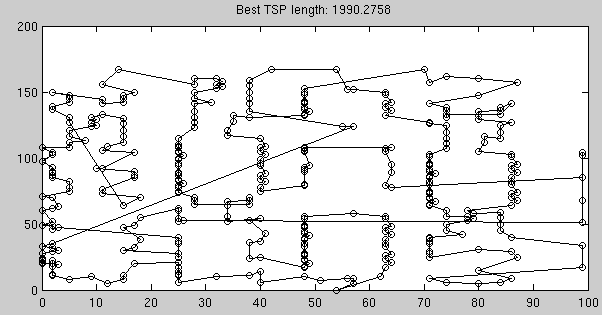
\includegraphics[width=0.5\textwidth]{bcl380_nn}
\caption[The nearest neighbor heuristic on \dataset{bcl380}.]{The nearest neighbor heuristic on \dataset{bcl380} shows it limitations: while overall a very good TSP solution, there are a few adverse stretches (built at the end of the construction of the path).}
\label{fig:bcl380_nn}
\end{figure}

\subsubsection{Simulated annealing}
\paragraph{Description}
Simulated annealing~\cite{simulatedannealing} (SA) is a generic probabilistic metaheuristic for the global optimization problem of locating a good approximation to the global optimum of a given function in a large search space. 
Wikipedia~\cite{sawiki} gives following description:
\begin{quote}
The name and inspiration come from annealing in metallurgy, a technique involving heating and controlled cooling of a material to increase the size of its crystals and reduce their defects. The heat causes the atoms to become unstuck from their initial positions (a local minimum of the internal energy) and wander randomly through states of higher energy; the slow cooling gives them more chances of finding configurations with lower internal energy than the initial one.

By analogy with this physical process, each step of the SA algorithm attempts to replace the current solution by a random solution (chosen according to a candidate distribution, often constructed to sample from solutions near the current solution). The new solution may then be accepted with a probability that depends both on the difference between the corresponding function values and also on a global parameter $T$ (called the temperature), that is gradually decreased during the process. The dependency is such that the choice between the previous and current solution is almost random when $T$ is large, but increasingly selects the better or ``downhill'' solution (for a minimization problem) as $T$ goes to zero. The allowance for ``uphill'' moves potentially saves the method from becoming stuck at local optima-which are the bane of greedier methods. 
\end{quote}


We initialized the TSP path for the simulated annealing algorithm\footnote{We used the simulated annealing toolbox found at \textsc{Matlab} File Exchange, \url{http://www.mathworks.com/matlabcentral/fileexchange/10548}.} with either a random path or one attained by the NN heuristic.  For neighborhood candidate solution generation, we simply used the exchange mutation operator. The initial temperature was 1, the cooling schedule was set so the temperature decreases with a factor $\beta=0.9$. Maximum consecutive rejections was set to 2500 and maximum tries to 500.
                              
\paragraph{Results}
Overall, we see very good results both solution quality wise as computational complexity wise. In general these algorithms require less parameters to set. The use of an path obtained by the NN heuristic as a initial solution for the simulated annealing algorithm does not result in significantly better solutions in the same parameter settings.

\clearpage
\section{Conclusion}
For the crossover operators, our results give the following hierarchies in performance: when considering speed, OX is definitely the fastest, followed by CX, and then PMX. The slowest are by far the powerful ERX and its even slower version EERX. 
When considering only the quality of the best solutions for the same number of allowed generations, the best crossover operators are clearly EERX and ERX. Next in order is the fast subtour preserving OX, followed by the position preserving PMX and CX. 
Overall, OX1 gives a good trade-off between solution quality and computational complexity.
%The hybrid crossover seems to perform averagely with respect to all the available crossover operators. 

Within the mutation operators, there were no real differences in solution quality nor time complexity. 
All four operators performed more or less the same. This shows that the choice of mutation operator is overall less important than the choice of the crossover operator.
% The results were more or less the same. When considering the computational speed however, we could deduce that the exchange mutation was the fastest operator, followed by the simple inversion, and next the slightly slower inversion which needs to calculate one extra pseudorandom number, and at last the slowest insertion mutation. 
%Again, the hybrid crossover is an average of the available operators.  

% The comparison of the three different selection operators also led to several conclusions. 
When comparing purely the selection operator, the differences in performance were again not very distinct. We could only see that the tournament selection operator works slightly slower than the stochastic uniform sampling and the proportional selection, which work at more or less the same speed. If we compared only the different selection operators, also no differences in solution quality came to view. However, the tournament selection seems to outperform the other operators when working in a high mutation environment. 

Considering the available crossover operators and mutation operators, it is very clear that the path representation is a massive improvement with respect to the adjacency representation. It is a more natural way of representing the phenotype of the tour, it allows crossover operators that have way better computational speeds, and it also allows operators that provide solutions that are much closer to the globally optimal solution. The path representation clearly outperforms the adjacency representation for the TSP problem. 

Comparing genetic algorithms with other approaches such as simulated annealing resulted in following interesting conclusion. In general, other heuristics such as SA or NN were easier to use and gave better solutions in less time.


\clearpage
\appendix
\section{\textsc{Matlab} code}
\label{sec:code}
\subsection{Crossover operators}
\label{appendix:crossover}
\subsubsection{PMX}
\lstinputlisting[firstline=32]{../../matlab/template/PMX_crossover.m}


\subsubsection{OX}
\lstinputlisting[firstline=30]{../../matlab/template/OX_crossover.m} 

\subsubsection{CX}
\lstinputlisting[firstline=29]{../../matlab/template/CX_crossover.m} 

\subsubsection{(E)ERX}
\lstinputlisting{../../matlab/template/edge_map.m} 
\lstinputlisting[firstline=29]{../../matlab/template/ERX_crossover.m} 
\lstinputlisting[firstline=29]{../../matlab/template/EERX_crossover.m} 




\subsection{Mutation operators} 
\label{appendix:mutation}
\subsubsection{Simple inversion}
\lstinputlisting[firstline=3]{../../matlab/template/simple_inversion.m} 

\subsubsection{Inversion}
\lstinputlisting[firstline=3]{../../matlab/template/inversion.m} 

\subsubsection{Insertion}
\lstinputlisting[firstline=3]{../../matlab/template/insertion.m} 

\subsubsection{Exchange}
\lstinputlisting[firstline=5]{../../matlab/template/exchange.m} 



\clearpage
\subsection{Selection operators} 
\label{appendix:selection}

\subsubsection{Tournament selection}
\lstinputlisting[firstline=2]{../../matlab/template/tournament_selection.m} 


\subsection{Other algorithms}
\subsubsection{Objective function}
\lstinputlisting[firstline=11]{../../matlab/template/tspfun.m} 
\subsubsection{Nearest neighbor heuristic}
\lstinputlisting{../../matlab/template/nn_heuristic.m} 

\clearpage

%% Define a new 'leo' style for the package that will use a smaller font.
\makeatletter
\def\url@leostyle{%
  \@ifundefined{selectfont}{\def\UrlFont{\sf}}{\def\UrlFont{\small\ttfamily}}}
\makeatother
%% Now actually use the newly defined style.
\urlstyle{leo}

\bibliography{biblio}


\end{document}

